\documentclass[11pt,aspectratio=169]{beamer}
\usetheme{Madrid}

% ======================= PACKAGES =======================
\usepackage{graphicx}
\usepackage{booktabs}
\usepackage{adjustbox}
\usepackage{multicol}
\usepackage{amsmath}
\usepackage{amssymb}
\usepackage{tikz}
\usetikzlibrary{arrows,shapes,positioning,shadows,trees}
\usepackage{listings}
\usepackage{xcolor}

% ======================= COLOR DEFINITIONS =======================
% Primary color scheme: Blue/Teal for Digital Finance
\definecolor{dfblue}{RGB}{0,102,204}
\definecolor{dfteal}{RGB}{0,153,153}
\definecolor{dfcyan}{RGB}{51,187,204}
\definecolor{dflightblue}{RGB}{153,204,255}
\definecolor{dflightblue2}{RGB}{173,214,255}
\definecolor{dflightblue3}{RGB}{193,224,255}
\definecolor{dflightblue4}{RGB}{213,234,255}

% Accent colors for finance applications
\definecolor{dfgreen}{RGB}{44, 160, 44}
\definecolor{dfred}{RGB}{214, 39, 40}
\definecolor{dforange}{RGB}{255, 127, 14}
\definecolor{dfgray}{RGB}{127, 127, 127}

% Utility colors
\definecolor{lightgray}{RGB}{240, 240, 240}
\definecolor{midgray}{RGB}{180, 180, 180}
\definecolor{codebg}{RGB}{245, 245, 245}

% ======================= THEME CUSTOMIZATION =======================
% Apply Digital Finance color scheme to Madrid theme
\setbeamercolor{palette primary}{bg=dflightblue3,fg=dfblue}
\setbeamercolor{palette secondary}{bg=dflightblue2,fg=dfblue}
\setbeamercolor{palette tertiary}{bg=dfteal,fg=white}
\setbeamercolor{palette quaternary}{bg=dfblue,fg=white}

\setbeamercolor{structure}{fg=dfblue}
\setbeamercolor{section in toc}{fg=dfblue}
\setbeamercolor{subsection in toc}{fg=dfteal}
\setbeamercolor{title}{fg=dfblue}
\setbeamercolor{frametitle}{fg=dfblue,bg=dflightblue3}
\setbeamercolor{block title}{bg=dflightblue2,fg=dfblue}
\setbeamercolor{block body}{bg=dflightblue4,fg=black}

% Remove navigation symbols for cleaner look
\setbeamertemplate{navigation symbols}{}

% Clean itemize/enumerate
\setbeamertemplate{itemize items}[circle]
\setbeamertemplate{enumerate items}[default]

% Margins for readability
\setbeamersize{text margin left=8mm,text margin right=8mm}

% ======================= LISTINGS CONFIGURATION =======================
% Python code style
\lstdefinestyle{pythonstyle}{
    language=Python,
    basicstyle=\ttfamily\footnotesize,
    keywordstyle=\color{dfblue}\bfseries,
    stringstyle=\color{dforange},
    commentstyle=\color{dfgray}\itshape,
    numberstyle=\tiny\color{dfgray},
    numbers=left,
    numbersep=5pt,
    backgroundcolor=\color{codebg},
    showspaces=false,
    showstringspaces=false,
    showtabs=false,
    frame=single,
    rulecolor=\color{midgray},
    tabsize=4,
    captionpos=b,
    breaklines=true,
    breakatwhitespace=false,
    escapeinside={(*@}{@*)},
    xleftmargin=10pt,
    xrightmargin=10pt
}

% Solidity code style
\lstdefinestyle{soliditystyle}{
    language=Java, % closest approximation
    basicstyle=\ttfamily\footnotesize,
    keywordstyle=\color{dfteal}\bfseries,
    stringstyle=\color{dforange},
    commentstyle=\color{dfgray}\itshape,
    numberstyle=\tiny\color{dfgray},
    numbers=left,
    numbersep=5pt,
    backgroundcolor=\color{codebg},
    showspaces=false,
    showstringspaces=false,
    showtabs=false,
    frame=single,
    rulecolor=\color{midgray},
    tabsize=2,
    captionpos=b,
    breaklines=true,
    breakatwhitespace=false,
    escapeinside={(*@}{@*)},
    xleftmargin=10pt,
    xrightmargin=10pt,
    morekeywords={pragma, contract, function, returns, public, private, view, pure, payable, address, uint256, mapping, event, modifier}
}

% Inline code command
\newcommand{\code}[1]{\texttt{\color{dfblue}#1}}

% ======================= CUSTOM COMMANDS =======================
% Bottom annotation (Madrid-style)
\newcommand{\bottomnote}[1]{%
\vfill
\vspace{-2mm}
\textcolor{dflightblue2}{\rule{\textwidth}{0.4pt}}
\vspace{1mm}
\footnotesize
\textbf{#1}
}

% Compact list spacing
\newcommand{\compactlist}{%
\setlength{\itemsep}{0pt}%
\setlength{\parskip}{0pt}%
\setlength{\parsep}{0pt}%
}

% Chart placeholder
\newcommand{\chartplaceholder}[2][5cm]{%
\begin{center}
\begin{adjustbox}{max width=0.95\textwidth, max height=#1}
\framebox[\textwidth][c]{%
\rule{0pt}{#1}%
\textcolor{midgray}{[#2]}%
}
\end{adjustbox}
\end{center}
}

% ======================= FINANCE NOTATION MACROS =======================
% Probability and statistics
\newcommand{\E}{\mathbb{E}} % Expected value
\newcommand{\Var}{\mathrm{Var}} % Variance
\newcommand{\Cov}{\mathrm{Cov}} % Covariance
\newcommand{\Prob}{\mathbb{P}} % Probability

% Distributions
\newcommand{\Normal}{\mathcal{N}} % Normal distribution
\newcommand{\Uniform}{\mathcal{U}} % Uniform distribution

% Returns and prices
\newcommand{\Ret}{R} % Return
\newcommand{\LogRet}{r} % Log return
\newcommand{\Price}{S} % Price/Stock price
\newcommand{\Strike}{K} % Strike price

% Options and derivatives
\newcommand{\CallPrice}{C} % Call option price
\newcommand{\PutPrice}{P} % Put option price
\newcommand{\Greeks}[1]{\mathit{#1}} % Greek letters

% Risk measures
\newcommand{\VaR}{\mathrm{VaR}} % Value at Risk
\newcommand{\CVaR}{\mathrm{CVaR}} % Conditional VaR
\newcommand{\Sharpe}{\mathrm{SR}} % Sharpe Ratio

% Time series
\newcommand{\AR}{\mathrm{AR}} % Autoregressive
\newcommand{\MA}{\mathrm{MA}} % Moving average
\newcommand{\GARCH}{\mathrm{GARCH}} % GARCH

% Blockchain/Crypto
\newcommand{\Hash}{\mathrm{Hash}} % Hash function
\newcommand{\Block}{\mathcal{B}} % Block
\newcommand{\Chain}{\mathcal{C}} % Chain

% Real numbers, integers
\newcommand{\R}{\mathbb{R}}
\newcommand{\Z}{\mathbb{Z}}
\newcommand{\N}{\mathbb{N}}

% ======================= TIKZ STYLES =======================
% Styles for finance-related diagrams
\tikzstyle{process} = [rectangle, minimum width=3cm, minimum height=1cm, text centered, draw=dfblue, fill=dflightblue4, thick]
\tikzstyle{decision} = [diamond, minimum width=3cm, minimum height=1cm, text centered, draw=dfteal, fill=dflightblue4, thick]
\tikzstyle{arrow} = [thick,->,>=stealth,color=dfblue]
\tikzstyle{blockchain} = [rectangle, rounded corners, minimum width=2.5cm, minimum height=1cm, text centered, draw=dfteal, fill=dflightblue3, thick]
\tikzstyle{transaction} = [circle, minimum size=0.8cm, text centered, draw=dforange, fill=dflightblue4, thick]

% ======================= FOOTER TEMPLATE =======================
\setbeamertemplate{footline}{
    \hbox{\begin{beamercolorbox}[wd=\paperwidth,ht=2.5ex,dp=1ex,leftskip=.5em,rightskip=.5em]{author in head/foot}
    \tiny
    \textbf{Digital Finance} \hfill
    Joerg Osterrieder \hfill
    \insertdate \hfill
    Page \insertframenumber{} / \inserttotalframenumber
    \end{beamercolorbox}}
}

% ======================= SECTION DIVIDER TEMPLATE =======================
\AtBeginSection[]{
\begin{frame}[plain]
\vfill
\centering
\begin{beamercolorbox}[sep=12pt,center]{title}
\usebeamerfont{title}\LARGE\insertsection\par
\end{beamercolorbox}
\vfill
\end{frame}
}


% ======================= DOCUMENT INFO =======================
\title{Topic 2.4: Platform Economics}
\subtitle{Network Effects, Winner-Take-Most, and FinTech Business Models}
\author{Joerg Osterrieder}
\institute{Digital Finance}
\date{}

\begin{document}

% ============================================================================
% SLIDE 1: Title
% ============================================================================
\begin{frame}[plain]
\titlepage
\end{frame}

% ============================================================================
% SLIDE 2: Learning Objectives
% ============================================================================
\begin{frame}{Learning Objectives}
\begin{block}{By the end of this topic, you will be able to:}
\begin{enumerate}
\item \textbf{Define} what a platform is and distinguish it from traditional pipeline businesses
\item \textbf{Explain} direct and indirect network effects using intuitive examples
\item \textbf{Analyze} winner-take-most dynamics and identify when markets ``tip''
\item \textbf{Evaluate} FinTech business models using conceptual frameworks for revenue and sustainability
\item \textbf{Assess} whether a FinTech's growth is sustainable or venture-subsidized
\item \textbf{Identify} regulatory moats and competitive barriers in financial services
\end{enumerate}
\end{block}

\vspace{3mm}
\begin{alertblock}{Key Competency}
Analyze a FinTech business model and assess its long-term sustainability using platform economics concepts.
\end{alertblock}
\end{frame}

% ============================================================================
% SLIDE 3: Prerequisites -- Economic Fundamentals
% ============================================================================
\begin{frame}{Prerequisites: Economic Fundamentals}
\textbf{Before we begin, let's establish some foundational concepts:}

\vspace{3mm}
\begin{columns}[T]
\begin{column}{0.5\textwidth}
\textbf{Supply and Demand:}
\begin{itemize}
\item Markets match buyers (demand) with sellers (supply)
\item Prices adjust to balance the two
\item Traditional economics assumes linear relationships
\end{itemize}

\vspace{3mm}
\textbf{Business Models:}
\begin{itemize}
\item How a company creates value
\item How a company captures value (revenue)
\item Who pays and who benefits
\end{itemize}
\end{column}
\begin{column}{0.5\textwidth}
\textbf{Key Terms to Know:}
\begin{itemize}
\item \textbf{Value Chain}: Steps to create and deliver a product
\item \textbf{Marginal Cost}: Cost of producing one more unit
\item \textbf{Economies of Scale}: Lower costs at higher volumes
\item \textbf{Intermediary}: A middleman connecting two parties
\end{itemize}

\vspace{3mm}
\textbf{Why This Matters:}\\
Platform economics \textit{changes} these traditional rules --- and understanding how is the key to evaluating modern FinTech
\end{column}
\end{columns}
\end{frame}

% ============================================================================
% SLIDE 4: The Shift from Making to Connecting
% ============================================================================
\begin{frame}{The Shift from Making to Connecting}
\begin{alertblock}{The Problem}
Why are some of the most valuable companies in the world ones that don't make anything?
\end{alertblock}

\vspace{3mm}
\begin{columns}[T]
\begin{column}{0.5\textwidth}
\textbf{The Concept:}
\begin{itemize}
\item Traditional businesses (``pipelines'') create value by \textbf{producing} goods or services and selling them along a linear chain
\item Modern platforms create value by \textbf{connecting} people who need each other
\item The shift: from owning factories to owning relationships
\end{itemize}

\vspace{3mm}
\begin{center}
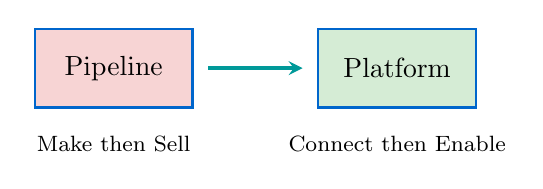
\begin{tikzpicture}[scale=0.8]
% Traditional
\node[process, fill=dfred!20, minimum width=2cm] (trad) at (0,2) {Pipeline};
\node[font=\footnotesize] at (0,0.8) {Make then Sell};

% Arrow
\draw[arrow, very thick, dfteal] (1.5,2) -- (3,2);

% Digital
\node[process, fill=dfgreen!20, minimum width=2cm] (dig) at (4.5,2) {Platform};
\node[font=\footnotesize] at (4.5,0.8) {Connect then Enable};
\end{tikzpicture}
\end{center}
\end{column}
\begin{column}{0.5\textwidth}
\textbf{In Finance:}
\begin{itemize}
\item A traditional bank \textit{manufactures} financial products (loans, accounts) and sells them through branches
\item A peer-to-peer lending platform \textit{connects} borrowers directly with investors who fund loans
\item A payment network \textit{connects} merchants with cardholders worldwide
\end{itemize}

\vspace{3mm}
\begin{block}{The Insight}
The most powerful business model of our era is connecting people, not producing goods. Platforms do not need to own inventory, branches, or factories --- they orchestrate transactions.
\end{block}
\end{column}
\end{columns}
\end{frame}

% ============================================================================
% SLIDE 5: What is a Platform?
% ============================================================================
\begin{frame}{What is a Platform?}
\begin{alertblock}{The Problem}
What makes a platform fundamentally different from a traditional business?
\end{alertblock}

\vspace{3mm}
\begin{columns}[T]
\begin{column}{0.5\textwidth}
\textbf{The Concept:}\\
A \textcolor{dfblue}{\textbf{platform}} is a business that creates value by facilitating exchanges between two or more interdependent groups.

\vspace{3mm}
\textbf{Key Characteristics:}
\begin{itemize}
\item Two or more distinct user groups
\item Each group needs the other to participate
\item The platform orchestrates and facilitates their interaction
\item Value is created by the participants, not the platform itself
\end{itemize}
\end{column}
\begin{column}{0.5\textwidth}
\begin{center}
\begin{adjustbox}{max width=\textwidth}
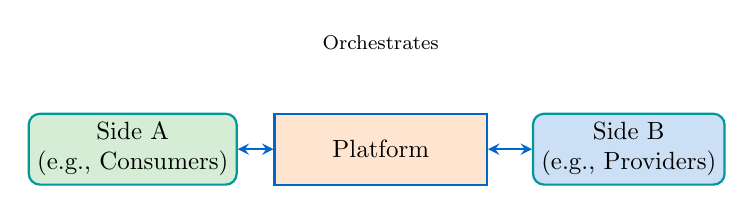
\begin{tikzpicture}[node distance=2cm, scale=0.9, transform shape]
% Platform model
\node (side1) [blockchain, fill=dfgreen!20, align=center] {Side A\\(e.g., Consumers)};
\node (platform) [process, right of=side1, xshift=1.5cm, fill=dforange!20] {Platform};
\node (side2) [blockchain, right of=platform, xshift=1.5cm, fill=dfblue!20, align=center] {Side B\\(e.g., Providers)};

% Arrows - bidirectional
\draw[thick, dfblue, stealth-stealth] (side1) -- (platform);
\draw[thick, dfblue, stealth-stealth] (platform) -- (side2);

% Value labels
\node[above of=platform, yshift=-0.5cm, font=\footnotesize] {Orchestrates};
\end{tikzpicture}
\end{adjustbox}
\end{center}

\vspace{5mm}
\begin{block}{The Insight}
Platforms don't own the means of production --- they own the means of \textbf{connection}. This is a fundamentally different source of power.
\end{block}
\end{column}
\end{columns}
\end{frame}

% ============================================================================
% SLIDE 6: Pipeline vs Platform Comparison
% ============================================================================
\begin{frame}{Pipeline vs.\ Platform: A Detailed Comparison}
\begin{center}
\begin{tabular}{p{3cm}p{5cm}p{5cm}}
\toprule
\textbf{Dimension} & \textbf{Pipeline (Traditional)} & \textbf{Platform (Digital)} \\
\midrule
\textbf{Value Creation} & Firm creates and sells products & Users create value for each other \\
\textbf{Assets} & Physical (branches, inventory) & Digital (software, data, networks) \\
\textbf{Growth} & Linear (more output = more cost) & Non-linear (network effects) \\
\textbf{Scalability} & Limited by physical capacity & Near-unlimited at low marginal cost \\
\textbf{Competition} & Product features and price & Ecosystem size and quality \\
\textbf{Moat} & Proprietary technology, brand & Network effects, data, switching costs \\
\bottomrule
\end{tabular}
\end{center}

\vspace{5mm}
\textbf{Examples in Finance:}
\begin{itemize}
\item \textbf{Pipeline}: A traditional bank manufactures loans and sells them to customers through branches
\item \textbf{Platform}: A peer-to-peer lending platform connects borrowers with investors who fund loans directly
\end{itemize}

\bottomnote{A \textbf{two-sided market} is a platform connecting two distinct groups who need each other.}
\end{frame}

% ============================================================================
% SLIDE 7: Network Effects -- The Core Mechanism
% ============================================================================
\begin{frame}{Network Effects: The Core Mechanism}
\begin{alertblock}{The Problem}
Why does a payment network become more useful as more people join it?
\end{alertblock}

\vspace{3mm}
\begin{columns}[T]
\begin{column}{0.5\textwidth}
\textbf{Direct (Same-Side) Network Effects:}\\
More users on the same side makes the platform more valuable for everyone on that side.

\vspace{2mm}
\textit{Example}: A peer payment app --- the more of your friends who use it, the more useful it is to you.

\vspace{5mm}
\textbf{Indirect (Cross-Side) Network Effects:}\\
More users on Side A makes the platform more attractive to Side B, and vice versa.

\vspace{2mm}
\textit{Example}: The more cardholders a card network has, the more merchants want to accept it --- and vice versa.
\end{column}
\begin{column}{0.5\textwidth}
\textbf{What is an Externality?}\\
When your action affects others who didn't choose to be affected. Network effects are a \textit{positive externality} --- each new user makes the platform better for all existing users.
\end{column}
\end{columns}
\end{frame}

% ============================================================================
\begin{frame}{Network Effects: The Core Mechanism (cont.)}
\begin{block}{The Insight}
Each new user adds value for \textit{all} existing users --- this is what makes platforms so powerful and why they invest so heavily in early growth.
\end{block}

\vspace{3mm}
\begin{alertblock}{Critical Question}
Does this company have \textbf{real} network effects, or just \textbf{growth}?\\
\vspace{2mm}
\textit{Growth without network effects is just expensive customer acquisition.}
\end{alertblock}
\end{frame}

% ============================================================================
% SLIDE 8: Why Networks Grow So Fast
% ============================================================================
\begin{frame}{Why Networks Grow So Fast}
\begin{alertblock}{The Problem}
Why do platforms seem to explode in growth once they reach a certain size?
\end{alertblock}

\vspace{3mm}
\begin{columns}[T]
\begin{column}{0.5\textwidth}
\textbf{The Concept:}
\begin{itemize}
\item In a traditional (linear) business, doubling your customers roughly doubles your value
\item In a network, doubling users \textbf{far more than doubles} the value --- because every new user can interact with every existing user
\item Network value grows much faster than the number of users
\end{itemize}

\vspace{3mm}
\textbf{Intuitive Example:}\\
A group chat with three friends has three possible conversations. Add a fourth friend, and suddenly there are six. Add a fifth, and there are ten. The connections multiply faster than the people.
\end{column}
\begin{column}{0.5\textwidth}
\begin{center}
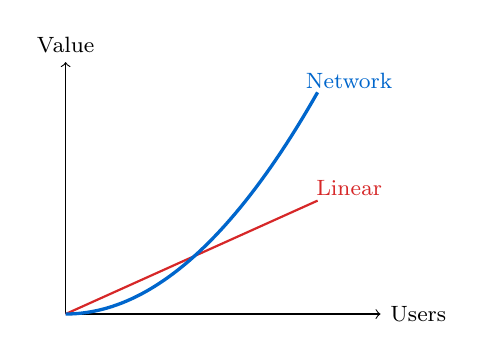
\begin{tikzpicture}[scale=0.8]
% Axes (no numbers)
\draw[->] (0,0) -- (5,0) node[right, font=\footnotesize] {Users};
\draw[->] (0,0) -- (0,4) node[above, font=\footnotesize] {Value};

% Linear growth
\draw[dfred, thick] (0,0) -- (4,1.8);
\node[dfred, font=\footnotesize] at (4.5,2) {Linear};

% Network growth (quadratic)
\draw[dfblue, very thick, domain=0:4, samples=50] plot (\x, {0.22*\x*\x});
\node[dfblue, font=\footnotesize] at (4.5,3.7) {Network};
\end{tikzpicture}
\end{center}
\end{column}
\end{columns}
\end{frame}

% ============================================================================
\begin{frame}{Why Networks Grow So Fast (cont.)}
\begin{block}{The Insight}
Doubling the number of users far more than doubles the value of a network. This is why platforms invest enormous sums in early growth --- the payoff compounds with every new user.
\end{block}
\end{frame}

% ============================================================================
% SLIDE 9: Types of Network Effects
% ============================================================================
\begin{frame}{Types of Network Effects in FinTech}
\begin{center}
\begin{tabular}{p{3cm}p{4.5cm}p{4.5cm}}
\toprule
\textbf{Type} & \textbf{Description} & \textbf{FinTech Pattern} \\
\midrule
\textbf{Direct} & Same-side: more users attract more users & Peer payment apps grow as friend groups join \\
\textbf{Indirect (Cross-side)} & One side attracts the other & Card networks: more cardholders attract more merchants \\
\textbf{Data Network Effects} & More users generate better algorithms & Lending platforms improve risk models with every loan \\
\textbf{Ecosystem Effects} & Third parties build on the platform & Payment processors attract developer tool ecosystems \\
\bottomrule
\end{tabular}
\end{center}

\vspace{3mm}
\textbf{The strongest FinTechs combine multiple types of network effects:}
\begin{itemize}
\item A payment processor benefits from indirect effects (merchants and consumers), data effects (better fraud detection), and ecosystem effects (developer tools)
\item A peer payment app may only have direct effects --- and that limits its defensibility
\end{itemize}

\bottomnote{\textbf{Disintermediation}: cutting out the middleman --- e.g., airlines selling tickets directly instead of through travel agents.}
\end{frame}

% ============================================================================
% SLIDE 10: The Chicken-and-Egg Problem
% ============================================================================
\begin{frame}{The Chicken-and-Egg Problem}
\begin{alertblock}{The Problem}
How do you launch a platform when each side needs the other to exist first?
\end{alertblock}

\vspace{3mm}
\begin{center}
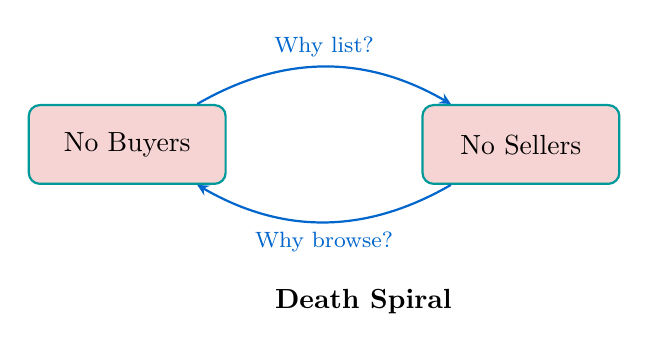
\begin{tikzpicture}[node distance=3cm]
% Death spiral
\node (no_buyers) [blockchain, fill=dfred!20] {No Buyers};
\node (no_sellers) [blockchain, right of=no_buyers, xshift=2cm, fill=dfred!20] {No Sellers};

\draw[arrow, bend left=30] (no_buyers) to node[above, font=\footnotesize] {Why list?} (no_sellers);
\draw[arrow, bend left=30] (no_sellers) to node[below, font=\footnotesize] {Why browse?} (no_buyers);

\node[below of=no_buyers, xshift=3cm, yshift=1cm, font=\bfseries] {Death Spiral};
\end{tikzpicture}
\end{center}
\end{frame}

% ============================================================================
\begin{frame}{The Chicken-and-Egg Problem (cont.)}
\textbf{Three Launch Strategies:}
\begin{columns}[T]
\begin{column}{0.33\textwidth}
\textbf{Subsidize One Side}\\
One early payment platform famously paid new users to join --- absorbing losses to reach critical mass quickly.
\end{column}
\begin{column}{0.33\textwidth}
\textbf{Single-Player Mode}\\
Make the product useful even without a network --- e.g., an app that tracks expenses alone but becomes more powerful when friends join.
\end{column}
\begin{column}{0.33\textwidth}
\textbf{Seed Supply}\\
Create initial supply yourself or partner with existing providers so the platform has value from day one.
\end{column}
\end{columns}

\vspace{3mm}
\begin{block}{The Insight}
Every successful platform found a creative way to solve this bootstrapping problem. The strategy chosen often shapes the platform's economics for years.
\end{block}
\end{frame}

% ============================================================================
% SLIDE 11: Critical Mass -- The Tipping Point
% ============================================================================
\begin{frame}{Critical Mass: The Tipping Point}
\begin{alertblock}{The Problem}
Why do some platforms succeed spectacularly while nearly identical ones fail completely?
\end{alertblock}

\vspace{2mm}
\begin{columns}[T]
\begin{column}{0.5\textwidth}
\textbf{The Concept:}\\
\textcolor{dfblue}{\textbf{Critical mass}} is the minimum number of users needed for a network to become self-sustaining.

\vspace{3mm}
\textbf{Below Critical Mass:}
\begin{itemize}
\item Users leave faster than they join
\item Value proposition is too weak
\item Requires constant subsidies to survive
\end{itemize}

\vspace{3mm}
\textbf{Above Critical Mass:}
\begin{itemize}
\item Organic growth accelerates on its own
\item Network effects compound
\item Winner-take-most dynamics begin
\end{itemize}
\end{column}
\begin{column}{0.5\textwidth}
\begin{center}
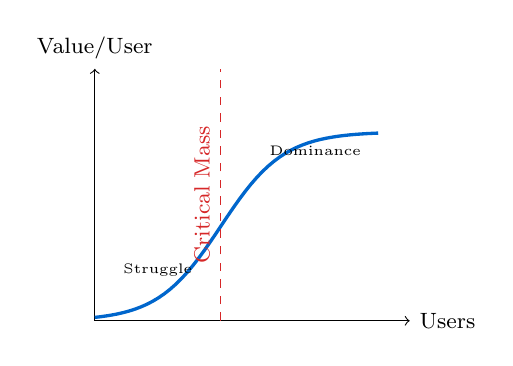
\begin{tikzpicture}[scale=0.8]
% Axes (no numbers)
\draw[->] (0,0) -- (5,0) node[right, font=\footnotesize] {Users};
\draw[->] (0,0) -- (0,4) node[above, font=\footnotesize] {Value/User};

% S-curve
\draw[dfblue, very thick, domain=0:4.5, samples=50] plot (\x, {3/(1+exp(-2*(\x-2)))});

% Critical mass line
\draw[dfred, dashed] (2,0) -- (2,4);
\node[dfred, font=\footnotesize, rotate=90] at (1.7,2) {Critical Mass};

% Labels
\node[font=\tiny] at (1,0.8) {Struggle};
\node[font=\tiny] at (3.5,2.7) {Dominance};
\end{tikzpicture}
\end{center}
\end{column}
\end{columns}
\end{frame}

% ============================================================================
\begin{frame}{Critical Mass: The Tipping Point (cont.)}
\begin{block}{The Insight}
Below critical mass, platforms collapse. Above it, they dominate. This is why FinTechs raise enormous amounts of venture capital --- to reach that tipping point before running out of money.
\end{block}
\end{frame}

% ============================================================================
% SLIDE 12: Winner-Take-Most Dynamics
% ============================================================================
\begin{frame}{Winner-Take-Most Dynamics}
\begin{alertblock}{The Problem}
Why do some markets end up with one dominant player while others sustain healthy competition?
\end{alertblock}

\vspace{1mm}
\begin{columns}[T]
\begin{column}{0.5\textwidth}
\textbf{The Concept:}\\
A market ``tips'' toward a single dominant player when three conditions align:

\vspace{1mm}
\begin{enumerate}\compactlist
\item \textbf{Strong network effects} --- each new user significantly increases value for all
\item \textbf{High switching costs} --- it is expensive or difficult to move to a competitor
\item \textbf{Low multi-homing} --- users find it impractical to use multiple platforms
\end{enumerate}

\vspace{1mm}
\textbf{Key Distinction:}
\begin{itemize}\compactlist
\item \textbf{Winner-take-all}: One company captures nearly the entire market
\item \textbf{Winner-take-most}: A dominant player emerges but competition survives at the margins
\end{itemize}
\end{column}
\begin{column}{0.5\textwidth}
\textbf{FinTech Examples:}
\begin{itemize}\compactlist
\item \textbf{Tips}: Card networks --- strong network effects, high switching costs for merchants
\item \textbf{Does not tip}: Neobanks --- low switching costs, easy to hold multiple accounts
\end{itemize}

\vspace{1mm}
\begin{block}{The Insight}
Not all markets tip --- understanding \textit{when} they do is the key to evaluating any FinTech investment. The conditions must all be present simultaneously.
\end{block}

\vspace{1mm}
\begin{alertblock}{Key Question}
Does this FinTech's market have the conditions to tip, or will competition persist?
\end{alertblock}
\end{column}
\end{columns}
\end{frame}

% ============================================================================
% SLIDE 13: Multi-Homing -- The Competition Preserver
% ============================================================================
\begin{frame}{Multi-Homing: The Competition Preserver}
\begin{alertblock}{The Problem}
What prevents a single platform from monopolizing a market?
\end{alertblock}

\vspace{1mm}
\textbf{The Concept:}\\
\textcolor{dfblue}{\textbf{Multi-homing}} means using multiple competing platforms simultaneously. When multi-homing is easy, no single platform can lock users in.

\vspace{1mm}
\begin{columns}[T]
\begin{column}{0.5\textwidth}
\textbf{Low Multi-Homing Costs:}
\begin{itemize}\compactlist
\item Easy to switch or use both platforms
\item Competition remains intense
\item No clear winner emerges
\item Pricing power stays limited
\end{itemize}

\vspace{2mm}
\textit{Pattern}: Ride-sharing, food delivery, buy-now-pay-later --- users freely switch between providers.
\end{column}
\begin{column}{0.5\textwidth}
\textbf{High Multi-Homing Costs:}
\begin{itemize}\compactlist
\item Expensive or difficult to switch
\item Users commit to one platform
\item Market tips toward a winner
\item The winner gains pricing power
\end{itemize}

\vspace{2mm}
\textit{Pattern}: Payment networks, enterprise software --- deep integration creates lock-in.
\end{column}
\end{columns}

\vspace{1mm}
\begin{block}{The Insight}
Successful platforms try to \textit{increase} switching costs to lock users in. Regulators try to \textit{decrease} them to preserve competition. Understanding this tension is central to platform strategy.
\end{block}
\end{frame}

% ============================================================================
% SLIDE 14: FinTech Business Model Canvas
% ============================================================================
\begin{frame}{FinTech Business Model Canvas}
\begin{alertblock}{The Problem}
How do you systematically analyze any FinTech's business model?
\end{alertblock}

\vspace{1mm}
\begin{center}
\begin{tabular}{p{3cm}p{4.5cm}p{4.5cm}}
\toprule
\textbf{Element} & \textbf{Key Questions} & \textbf{What to Look For} \\
\midrule
\textbf{Value Proposition} & What pain point does it solve? How is it better than alternatives? & Speed, cost, access, user experience \\
\textbf{Revenue Model} & Who pays? For what? How often? & Transaction fees, subscriptions, interest, data \\
\textbf{Cost Structure} & What are the major costs? Do they scale? & Acquisition, infrastructure, compliance \\
\textbf{Network Effects} & Direct? Indirect? Data flywheel? & User-to-user, cross-side, algorithmic \\
\textbf{Moat} & What prevents competitors from copying this? & Switching costs, data, regulation \\
\textbf{Scalability} & Does the cost of serving one more customer approach zero? & Software vs.\ human-dependent \\
\bottomrule
\end{tabular}
\end{center}

\vspace{3mm}
\begin{block}{The Insight}
Use this framework to analyze any FinTech company systematically --- it separates hype from substance.
\end{block}
\end{frame}

% ============================================================================
% SLIDE 15: Revenue Models in FinTech
% ============================================================================
\begin{frame}{Revenue Models in FinTech}
\begin{alertblock}{The Problem}
How do FinTechs actually make money, especially when many products appear ``free''?
\end{alertblock}

\vspace{1mm}
\begin{columns}[T]
\begin{column}{0.5\textwidth}
\textbf{Transaction-Based:}
\begin{itemize}\compactlist
\item A small percentage of each transaction plus a flat fee
\item Interchange revenue from card spending
\item Foreign exchange markups on currency conversion
\end{itemize}

\vspace{1mm}
\textbf{Subscription:}
\begin{itemize}\compactlist
\item Premium tiers with additional features
\item Business-to-business software-as-a-service
\item Membership models with bundled services
\end{itemize}
\end{column}
\begin{column}{0.5\textwidth}
\textbf{Interest and Float:}
\begin{itemize}\compactlist
\item Earning interest on customer deposits held temporarily
\item Lending margin: borrow at a low rate, lend at a higher rate
\item Holding funds in transit and earning interest on the ``float''
\end{itemize}

\vspace{1mm}
\textbf{Data and Ecosystem:}
\begin{itemize}\compactlist
\item Selling order flow to market makers
\item Cross-selling additional products to existing customers
\item Licensing aggregated, anonymized insights
\end{itemize}
\end{column}
\end{columns}

\vspace{1mm}
\begin{block}{The Insight}
The most resilient FinTechs combine multiple revenue streams. Dependence on a single source creates vulnerability --- especially if regulators restrict it.
\end{block}
\end{frame}

% ============================================================================
% SLIDE 16: Unit Economics -- Health Check
% ============================================================================
\begin{frame}{Unit Economics: The Health Check}
\begin{alertblock}{The Problem}
How do you tell if a fast-growing company is actually healthy --- or just burning money?
\end{alertblock}

\vspace{3mm}
\begin{columns}[T]
\begin{column}{0.5\textwidth}
\textbf{Key Concepts (No Math Required):}
\begin{itemize}
\item \textbf{CAC} (Customer Acquisition Cost): How much you spend to get one new customer
\item \textbf{LTV} (Lifetime Value): Total revenue expected from one customer over their entire relationship
\item \textbf{Payback Period}: How long until a customer ``pays back'' their acquisition cost
\item \textbf{Churn}: The rate at which customers leave
\end{itemize}

\vspace{3mm}
\textbf{The Core Question:}\\
Does each customer eventually pay back \textit{more} than it cost to acquire them?
\end{column}
\begin{column}{0.5\textwidth}
\textbf{Healthy vs.\ Unhealthy:}
\begin{itemize}
\item Lifetime value should be \textbf{several times} the acquisition cost
\item Payback should happen within a \textbf{reasonable timeframe}
\item Churn should be \textbf{low enough} that customers stay long enough to generate returns
\end{itemize}
\end{column}
\end{columns}
\end{frame}

% ============================================================================
\begin{frame}{Unit Economics: The Health Check (cont.)}
\begin{block}{FinTech CAC Challenges}
\begin{itemize}
\item Trust is required for financial products
\item Regulatory constraints limit marketing channels
\item High-intent keywords are expensive
\item Referral programs can be costly
\end{itemize}
\end{block}

\vspace{3mm}
\begin{block}{The Insight}
Growth without healthy unit economics is just burning money. Always ask: is each new customer profitable, or is the company paying more to acquire them than they will ever earn back?
\end{block}
\end{frame}

% ============================================================================
% SLIDE 17: Venture Subsidies -- Real or Fake Growth?
% ============================================================================
\begin{frame}{Venture Subsidies: Real Growth or Fake Economics?}
\begin{alertblock}{The Problem}
If a product is free or extremely cheap, is the demand real --- or artificial?
\end{alertblock}

\vspace{3mm}
\begin{columns}[T]
\begin{column}{0.5\textwidth}
\textbf{The Blitzscaling Playbook:}
\begin{enumerate}
\item Raise large amounts of venture capital
\item Use it to subsidize user acquisition (below-cost pricing, free products, sign-up bonuses)
\item Grow at all costs to reach critical mass
\item Achieve network effects and lock-in
\item Raise prices once dominant
\end{enumerate}
\end{column}
\begin{column}{0.5\textwidth}
\textbf{When This Works:}
\begin{itemize}
\item The market truly tips (winner-take-most)
\item Network effects create lasting value
\item Switching costs prevent users from leaving when prices rise
\end{itemize}
\end{column}
\end{columns}
\end{frame}

% ============================================================================
\begin{frame}{Venture Subsidies: Real Growth or Fake Economics? (cont.)}
\begin{alertblock}{When It Doesn't Work}
\begin{itemize}
\item Multi-homing prevents lock-in
\item No real network effects to capture
\item Regulation prevents pricing power
\item Competition never stops --- multiple players survive indefinitely
\end{itemize}
\end{alertblock}

\vspace{3mm}
\begin{block}{The ``Remove Subsidies'' Test}
\textbf{Ask}: Would customers stay at \textit{sustainable} prices?\\
\textbf{Test}: Mentally remove the subsidies --- what happens to demand?\\
\textbf{If demand collapses}: The growth was artificial.
\end{block}

\vspace{3mm}
\begin{block}{The Insight}
Always ask: would customers stay at sustainable prices? If the answer is unclear, the company may be building on sand.
\end{block}
\end{frame}

% ============================================================================
% SLIDE 18: The Data Flywheel in Platforms
% ============================================================================
\begin{frame}{The Data Flywheel in Platforms}
\begin{alertblock}{The Problem}
Why do data-rich platforms keep getting stronger while newcomers struggle to catch up?
\end{alertblock}

\vspace{3mm}
\begin{center}
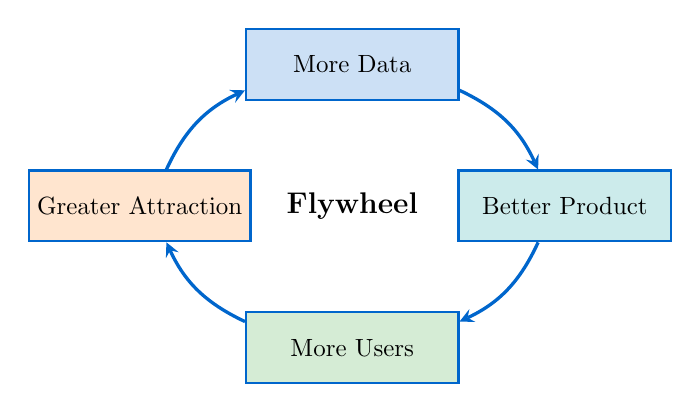
\begin{tikzpicture}[scale=0.9, transform shape]
% Flywheel nodes
\node (data) [process, fill=dfblue!20] at (0,2) {More Data};
\node (product) [process, fill=dfteal!20] at (3,0) {Better Product};
\node (users) [process, fill=dfgreen!20] at (0,-2) {More Users};
\node (attract) [process, fill=dforange!20] at (-3,0) {Greater Attraction};

% Arrows forming cycle
\draw[arrow, very thick] (data) to[bend left=20] (product);
\draw[arrow, very thick] (product) to[bend left=20] (users);
\draw[arrow, very thick] (users) to[bend left=20] (attract);
\draw[arrow, very thick] (attract) to[bend left=20] (data);

% Center label
\node[font=\large\bfseries] at (0,0) {Flywheel};
\end{tikzpicture}
\end{center}
\end{frame}

% ============================================================================
\begin{frame}{The Data Flywheel in Platforms (cont.)}
\textbf{How It Works in FinTech:}
\begin{itemize}
\item More transactions generate more data, which improves fraud detection, which reduces false declines, which attracts more merchants, which generates more transactions
\item More loan applications improve risk models, which enable more accurate pricing, which attracts better borrowers, which generates more data
\end{itemize}

\begin{block}{The Insight}
The data flywheel creates compounding advantages that new entrants cannot easily replicate --- it is one of the most powerful moats in modern finance.
\end{block}
\end{frame}

% ============================================================================
% SLIDE 19: Regulation as Moat
% ============================================================================
\begin{frame}{Regulation as Moat}
\begin{alertblock}{The Problem}
Can government rules actually \textit{help} a company rather than hurt it?
\end{alertblock}

\vspace{3mm}
\textbf{The Concept:}\\
Regulatory requirements (banking charters, insurance licenses, broker-dealer registrations, money transmitter licenses) are expensive and time-consuming to obtain.

\vspace{3mm}
\textbf{How Regulation Becomes a Moat:}
\begin{itemize}
\item Competitors must also obtain licenses
\item Time to comply creates a head start
\item Relationships with regulators are valuable
\item Compliance infrastructure, once built, is hard to replicate
\end{itemize}
\end{frame}

% ============================================================================
\begin{frame}{Regulation as Moat (cont.)}
\textbf{How FinTechs Navigate Regulation:}
\begin{itemize}
\item \textbf{Rent}: Use BaaS partnerships to operate under a partner bank's charter
\item \textbf{Obtain}: Apply for their own licenses (expensive but independent)
\item \textbf{Avoid}: Operate in less-regulated niches (risky long-term)
\end{itemize}

\vspace{3mm}
\begin{block}{The Insight}
Once compliant, regulation becomes a competitive barrier. It is expensive to achieve but creates a powerful moat that protects from new entrants.
\end{block}

\vspace{3mm}
\begin{alertblock}{The Double Edge}
Regulatory capture can flip: what protects you today can also restrict you tomorrow.
\end{alertblock}
\end{frame}

% ============================================================================
% SLIDE 20: How Incumbents Fight Back
% ============================================================================
\begin{frame}{How Incumbents Fight Back}
\begin{alertblock}{The Problem}
What do traditional banks and financial institutions do when FinTechs attack their business?
\end{alertblock}

\vspace{3mm}
\begin{center}
\begin{tabular}{p{2.5cm}p{4cm}p{4cm}}
\toprule
\textbf{Strategy} & \textbf{Advantages} & \textbf{Disadvantages} \\
\midrule
\textbf{Build} (Internal) & Full control, deep integration & Slow, cultural mismatch \\
\textbf{Buy} (Acquire) & Speed, talent, customer base & Expensive, integration risk \\
\textbf{Partner} (API/BaaS) & Fast to market, low commitment & Dependency, shared margins \\
\textbf{Copy} (Fast follow) & Proven concept, lower risk & Always behind, no differentiation \\
\textbf{Invest} (Minority stake) & Option value, market intelligence & Limited control \\
\bottomrule
\end{tabular}
\end{center}

\vspace{3mm}
\begin{block}{The Insight}
Traditional banks have significant advantages: trust, large deposit bases, existing customer relationships, and regulatory standing. But they often struggle with speed and cultural adaptation. The most effective response depends on the specific threat.
\end{block}
\end{frame}

% ============================================================================
% SLIDE 21: Case Pattern -- Commission-Free Trading
% ============================================================================
\begin{frame}{Case Pattern: Commission-Free Trading}
\begin{alertblock}{The Problem}
How can a trading app offer ``free'' trades --- and what is the hidden business model?
\end{alertblock}

\vspace{1mm}
\begin{columns}[T]
\begin{column}{0.55\textwidth}
\textbf{The Concept: Payment for Order Flow (PFOF)}
\begin{center}
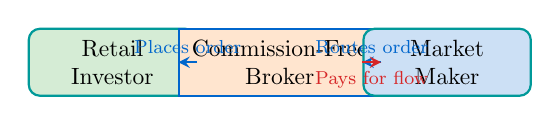
\begin{tikzpicture}[node distance=2.5cm, scale=0.85, transform shape]
\node (user) [blockchain, fill=dfgreen!20, align=center] {Retail\\Investor};
\node (broker) [process, right of=user, fill=dforange!20, align=center] {Commission-Free\\Broker};
\node (maker) [blockchain, right of=broker, fill=dfblue!20, align=center] {Market\\Maker};

\draw[arrow] (user) -- node[above, font=\footnotesize] {Places order} (broker);
\draw[arrow] (broker) -- node[above, font=\footnotesize] {Routes order} (maker);
\draw[arrow, dfred] (maker) -- node[below, font=\footnotesize] {Pays for flow} (broker);
\end{tikzpicture}
\end{center}

\vspace{2mm}
\textbf{How It Works:}
\begin{enumerate}\compactlist
\item You place a trade (no commission charged)
\item The broker routes your order to a market maker
\item The market maker pays the broker for that order flow
\item The market maker profits from the bid-ask spread
\end{enumerate}
\end{column}
\begin{column}{0.45\textwidth}
\textbf{Arguments For:}
\begin{itemize}\compactlist
\item Enables ``free'' trading for small investors
\item Price improvement may still occur
\item Democratizes access to markets
\end{itemize}

\vspace{1mm}
\textbf{Arguments Against:}
\begin{itemize}\compactlist
\item Hidden cost embedded in execution quality
\item Conflict of interest: whose interests come first?
\item Some regulators have restricted or banned it
\end{itemize}

\vspace{1mm}
\begin{block}{The Insight}
``Free'' products always have a hidden business model. When you are not paying for the product, you are likely the product --- or your order flow is.
\end{block}
\end{column}
\end{columns}
\end{frame}

% ============================================================================
% SLIDE 22: Discussion -- Evaluating FinTech Sustainability
% ============================================================================
\begin{frame}{Discussion: Evaluating FinTech Sustainability}
\begin{block}{Framework: Six Questions for Any FinTech}
\begin{enumerate}
\item Does this FinTech have \textbf{real network effects}, or just growth fueled by subsidies?
\item Are the \textbf{unit economics healthy} --- does each customer pay back more than they cost to acquire?
\item Are \textbf{switching costs} high enough to retain users when prices rise?
\item Does the \textbf{data advantage} compound over time via a flywheel?
\item Can incumbents \textbf{easily copy this} --- or is there a lasting moat?
\item Will \textbf{regulation} help or hurt the company long-term?
\end{enumerate}
\end{block}

\vspace{3mm}
\textbf{Discussion Exercise:}\\
Think about a financial app you use regularly. Apply these six questions:
\begin{itemize}
\item What would happen if the app raised its prices significantly?
\item Could you easily switch to an alternative? Would you?
\item Does the app get better the more people use it, or is the experience the same regardless?
\end{itemize}

\vspace{2mm}
\textit{There are no wrong answers --- the goal is to practice the framework.}
\end{frame}

% ============================================================================
% SLIDE 23: Executive Summary
% ============================================================================
\begin{frame}{Executive Summary: Key Takeaways}
\begin{enumerate}
\item \textbf{Platforms create value differently}: They orchestrate exchanges rather than produce goods --- the most powerful FinTechs are platforms, not pipelines

\item \textbf{Network effects are the goal, but not guaranteed}: Not every FinTech has real network effects --- growth without them is just expensive customer acquisition that evaporates when subsidies end

\item \textbf{Winner-take-most requires specific conditions}: Strong network effects combined with high switching costs and low multi-homing --- without all three, competition persists

\item \textbf{Unit economics determine sustainability}: Lifetime value should be several times the acquisition cost --- venture subsidies mask reality until funding stops

\item \textbf{Multiple moats beat single advantages}: The strongest FinTechs combine network effects, data flywheels, switching costs, and regulatory positioning
\end{enumerate}

\vspace{3mm}
\begin{block}{Core Skill}
Always ask: ``Would this business work at \textit{sustainable} prices without subsidies?''
\end{block}
\end{frame}

% ============================================================================
% SLIDE 24: Concept Map
% ============================================================================
\begin{frame}{Concept Map: Platform Economics}
\begin{center}
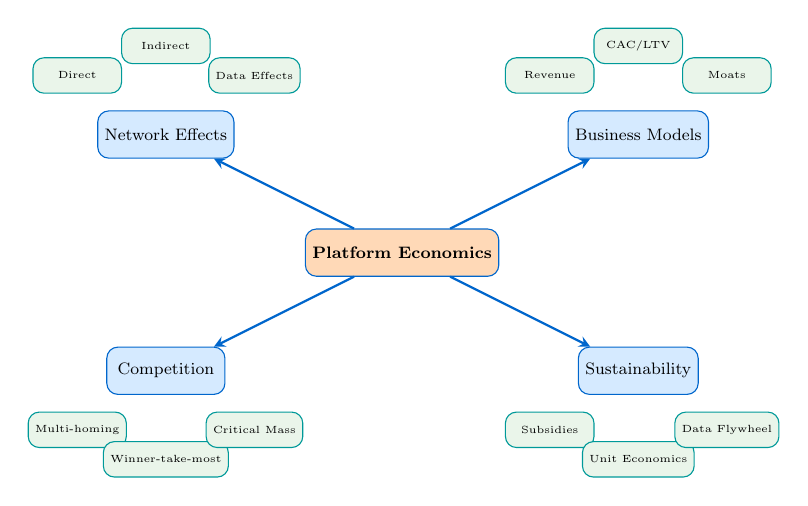
\begin{tikzpicture}[scale=0.75, transform shape,
    concept/.style={rectangle, rounded corners, draw=dfblue, fill=dflightblue4, minimum width=2cm, minimum height=0.8cm, font=\footnotesize},
    subcon/.style={rectangle, rounded corners, draw=dfteal, fill=dfgreen!10, minimum width=1.5cm, minimum height=0.6cm, font=\tiny}]

% Central concept
\node[concept, fill=dforange!30, minimum width=3cm] (platform) at (0,0) {\textbf{Platform Economics}};

% Main branches
\node[concept] (network) at (-4,2) {Network Effects};
\node[concept] (business) at (4,2) {Business Models};
\node[concept] (competition) at (-4,-2) {Competition};
\node[concept] (sustainability) at (4,-2) {Sustainability};

% Connect to center
\draw[arrow] (platform) -- (network);
\draw[arrow] (platform) -- (business);
\draw[arrow] (platform) -- (competition);
\draw[arrow] (platform) -- (sustainability);

% Sub-concepts
\node[subcon] at (-5.5,3) {Direct};
\node[subcon] at (-4,3.5) {Indirect};
\node[subcon] at (-2.5,3) {Data Effects};

\node[subcon] at (2.5,3) {Revenue};
\node[subcon] at (4,3.5) {CAC/LTV};
\node[subcon] at (5.5,3) {Moats};

\node[subcon] at (-5.5,-3) {Multi-homing};
\node[subcon] at (-4,-3.5) {Winner-take-most};
\node[subcon] at (-2.5,-3) {Critical Mass};

\node[subcon] at (2.5,-3) {Subsidies};
\node[subcon] at (4,-3.5) {Unit Economics};
\node[subcon] at (5.5,-3) {Data Flywheel};

\end{tikzpicture}
\end{center}
\end{frame}

% ============================================================================
% SLIDE 25: Key Terms
% ============================================================================
\begin{frame}{Key Terms and Definitions}
\begin{description}
\item[Platform] A business that creates value by facilitating exchanges between two or more interdependent groups
\item[Network Effect] When the value of a product or service increases as more people use it
\item[Critical Mass] The minimum number of users needed for a network to become self-sustaining
\item[Multi-Homing] Using multiple competing platforms simultaneously; when easy, it prevents monopoly
\item[Winner-Take-Most] Market dynamics where one platform captures a dominant share due to network effects, switching costs, and low multi-homing
\item[CAC] Customer Acquisition Cost --- total marketing spend to acquire one new customer
\item[LTV] Lifetime Value --- total revenue expected from a customer over their entire relationship
\item[Data Flywheel] A virtuous cycle where more data improves the product, attracting more users, generating more data
\item[Blitzscaling] Strategy of prioritizing rapid growth over efficiency to capture network effects quickly
\end{description}
\end{frame}

% ============================================================================
% SLIDE 26: Common Misconceptions + Self-Assessment
% ============================================================================
\begin{frame}{Common Misconceptions and Self-Assessment}
\begin{columns}[T]
\begin{column}{0.5\textwidth}
\textbf{Myth vs.\ Reality:}

\vspace{2mm}
\textbf{Myth}: ``All fast-growing FinTechs have network effects.''\\
\textbf{Reality}: Growth can come from subsidies alone. True network effects mean each new user makes the product more valuable for existing users.

\vspace{3mm}
\textbf{Myth}: ``Commission-free trading is truly free.''\\
\textbf{Reality}: Revenue comes from order flow payments. The cost is hidden in execution quality.

\vspace{3mm}
\textbf{Myth}: ``First mover always wins in platforms.''\\
\textbf{Reality}: A better-funded or better-designed later entrant can overtake. What matters is reaching critical mass and building switching costs.

\vspace{3mm}
\textbf{Myth}: ``More features means a stronger moat.''\\
\textbf{Reality}: Features can be copied. Moats come from network effects, data advantages, and switching costs.
\end{column}
\begin{column}{0.5\textwidth}
\textbf{Self-Assessment Questions:}

\vspace{3mm}
\textbf{Q1}: A peer-to-peer payment app has strong \underline{\hspace{2cm}} network effects because its value increases as more friends join.
\begin{itemize}
\item[A.] Indirect
\item[B.] Direct
\item[C.] Data
\item[D.] Ecosystem
\end{itemize}

\vspace{3mm}
\textbf{Q2}: Which condition does \textit{not} typically lead to winner-take-most dynamics?
\begin{itemize}
\item[A.] Strong network effects
\item[B.] Low multi-homing costs
\item[C.] High switching costs
\item[D.] Compounding data advantages
\end{itemize}

\vspace{3mm}
\textit{Answers: Q1 = B (Direct), Q2 = B (Low multi-homing costs prevent tipping because users can switch easily)}
\end{column}
\end{columns}
\end{frame}

% ============================================================================
% SLIDE 27: What's Next + Questions
% ============================================================================
\begin{frame}
\centering
\vspace{1cm}
{\Large \textbf{What's Next: Day 3 --- Blockchain Fundamentals}}

\vspace{5mm}
\begin{columns}[T]
\begin{column}{0.5\textwidth}
\textbf{Coming Up:}
\begin{itemize}
\item What is a blockchain and why does it matter?
\item Distributed ledger technology
\item Consensus mechanisms
\item Cryptographic foundations
\item Bitcoin, Ethereum, and smart contracts
\end{itemize}
\end{column}
\begin{column}{0.5\textwidth}
\textbf{Connection to Platform Economics:}
\begin{itemize}
\item Blockchain platforms have network effects too
\item Token incentives as a launch strategy
\item Can decentralized platforms compete with centralized ones?
\end{itemize}
\end{column}
\end{columns}

\vspace{8mm}
{\Huge Questions?}

\vspace{5mm}
{\normalsize Topic 2.4: Platform Economics --- Network Effects, Winner-Take-Most, and FinTech Business Models}

\vspace{3mm}
\textit{``Understanding platform economics is essential for evaluating which innovations are sustainable and which are built on venture subsidies.''}
\end{frame}

\end{document}
